% ============================================================
%  Chapter 8 -- Simulation of Queues and Related Models
%  Leskelä & Vihola: Lectures on Monte Carlo Theory
% ============================================================
\documentclass[aspectratio=169,10pt]{beamer}

\usetheme{Madrid}
\usecolortheme{seahorse}

\usepackage{amsmath,amssymb,amsfonts}
\usepackage{mathtools}
\usepackage{listings}
\usepackage{xcolor}
\usepackage{graphicx}
\usepackage{booktabs}
\usepackage{tikz}
\usepackage{array}

\graphicspath{{figures/}}

% ── Python listing style ──────────────────────────────────
\lstdefinestyle{python}{
  language=Python,
  basicstyle=\ttfamily\scriptsize,
  numbers=left,
  numberstyle=\tiny\color{gray},
  frame=single,
  backgroundcolor=\color{gray!7},
  keywordstyle=\color{blue!70!black}\bfseries,
  commentstyle=\color{green!50!black}\itshape,
  stringstyle=\color{orange!80!black},
  showstringspaces=false,
  breaklines=true,
  tabsize=4,
}

\setbeamertemplate{footline}[frame number]
\setbeamertemplate{navigation symbols}{}

% ── Math shortcuts ────────────────────────────────────────
\newcommand{\E}{\mathbb{E}}
\newcommand{\Var}{\mathbb{V}\mathrm{ar}}
\newcommand{\Prob}{\mathbb{P}}
\newcommand{\R}{\mathbb{R}}
\newcommand{\N}{\mathbb{N}}

% ============================================================
\title[Ch.8: Simulation of Queues]{Chapter 8\\Simulation of Queues and Related Models}
\subtitle{Lectures on Monte Carlo Theory}
\author{Leskel\"{a} \& Vihola}
\date{}

\begin{document}

\begin{frame}
  \titlepage
\end{frame}

% ── Table of Contents ─────────────────────────────────────
\begin{frame}{Chapter Overview}
  \tableofcontents
\end{frame}

% ============================================================
\section{8.1 Preliminaries}
% ============================================================

\begin{frame}{8.1 Preliminaries -- Queueing Systems}
  \textbf{A ``system'' receives tasks and processes them:}
  \begin{itemize}
    \item Tasks (jobs, customers, calls) arrive according to some mechanism.
    \item Tasks are processed in some manner and eventually leave.
  \end{itemize}
  \vspace{0.5em}
  \textbf{Two representations of system characteristics:}
  \begin{itemize}
    \item \emph{Discrete-time sequence}: e.g.\ waiting time $W_i$ of the $i$-th arriving task.
    \item \emph{Continuous-time process}: e.g.\ number of tasks $L(t)$ in the system at time $t$.
  \end{itemize}
\end{frame}

\begin{frame}{Time Averages vs.\ Ensemble Averages}
  \begin{block}{Time Average}
    For a process $X(t)$, the \emph{time average} over $[0,t]$ is:
    \[
      \hat{X}(t) = \frac{1}{t}\int_0^t X(s)\,ds.
    \]
    Represents the average value observed in a single long simulation run.
  \end{block}

  \begin{block}{Ensemble Average}
    The \emph{ensemble average} at time $t$ is $\E[X(t)]$, the expected value over all
    possible realizations.
  \end{block}

  \vspace{0.5em}
  \textbf{Key question:} When do $\hat{X}(t) \to \E[X^*]$ as $t\to\infty$?
  \begin{itemize}
    \item $X^*$ is a random variable with the \emph{stationary distribution}.
    \item Answer: when the process is \emph{ergodically stable} (Section 8.7).
  \end{itemize}
\end{frame}

\begin{frame}{Steady-State Characteristics}
  \begin{block}{Steady-State Mean and Variance}
    For a \emph{continuous-time} process $X(t)$ with stationary distribution:
    \[
      \E[X^*] = \lim_{t\to\infty}\frac{1}{t}\int_0^t X(s)\,ds,\qquad
      \Var[X^*] = \lim_{t\to\infty}\frac{1}{t}\int_0^t (X(s)-\E[X^*])^2\,ds.
    \]
  \end{block}

  For \emph{discrete-time} chains $(X_k)$ the analogues are:
  \[
    \mu = \E[X^*] = \lim_{k\to\infty}\frac{1}{k}\sum_{j=1}^k X_j,\qquad
    \sigma^2 = \Var[X^*] = \lim_{k\to\infty}\frac{1}{k}\sum_{j=1}^k X_j^2 - \mu^2.
  \]

  \textbf{Biased estimators from a single run:}
  \[
    \hat\mu(k) = \frac{1}{k}\sum_{j=1}^k X_j, \qquad
    \hat\sigma^2(k) = \frac{1}{k}\sum_{j=1}^k (X_j - \hat\mu(k))^2.
  \]
\end{frame}

% ============================================================
\section{8.2 Modeling Arrival Streams}
% ============================================================

\begin{frame}{8.2 Modeling Arrival Streams}
  \textbf{Counting process $N(t)$:}
  \begin{itemize}
    \item $N(t)$ = number of arrivals up to time $t$ ($t\ge 0$).
    \item Piecewise constant, non-decreasing, unit jumps; $N(0)=0$.
    \item Right-continuous in $t$.
  \end{itemize}

  \vspace{0.5em}
  \textbf{Arrival times $(A_n)$ and inter-arrival times $(\tau_i)$:}
  \begin{block}{Inter-Arrival Times and Counting Process}
    \[
      \tau_1 = A_1,\quad \tau_i = A_i - A_{i-1},\quad (i=2,\ldots)
      \tag{8.2.1}
    \]
    \[
      N(t) = \#\{i\ge 1 : A_i \le t\}.
      \tag{8.2.2}
    \]
    $\tau_i$ = inter-arrival times; $A_n$ = arrival instants.
  \end{block}

  \begin{block}{Interval Counts}
    For $s < t$:\quad $N(s,t] := N(t) - N(s) = \#\{i\ge 1: s < A_i \le t\}$.
  \end{block}
\end{frame}

% ── 8.2.1 ────────────────────────────────────────────────
\subsection{8.2.1 Homogeneous Poisson Process}

\begin{frame}{8.2.1 Homogeneous Poisson Process}
  \begin{block}{Definition 8.2.1}
    A counting process $N(t)$ is a \textbf{homogeneous Poisson process} with
    intensity $\lambda>0$ if the inter-arrival times $(\tau_j)$ are i.i.d.\
    $\mathrm{Exp}(\lambda)$.
  \end{block}

  \begin{block}{Proposition 8.2.2 (Equivalent Characterization)}
    $N(t)$ is a Poisson process with intensity $\lambda$ iff:
    \begin{enumerate}
      \item Numbers of points in disjoint intervals are \emph{independent}.
      \item $N(t,t+h] \sim \mathrm{Poi}(\lambda h)$ for all $t,h>0$.
    \end{enumerate}
  \end{block}

  \vspace{0.3em}
  \textbf{Key facts:}
  \begin{itemize}
    \item $N(t) \sim \mathrm{Poiss}(\lambda t)$.
    \item $\Prob(N(t,t+h]=1) = \lambda h e^{-\lambda h} = \lambda h + o(h)$.
    \item $\lambda$ = average arrival rate per unit time.
    \item Arrival times: $A_i = \tau_1 + \cdots + \tau_i$.
  \end{itemize}
\end{frame}

\begin{frame}{Simulation of Homogeneous Poisson Process}
  \begin{columns}
    \column{0.48\textwidth}
    \begin{block}{Algorithm PoiPro($\lambda$)}
      \footnotesize
      \begin{enumerate}
        \item Create empty list \texttt{A}
        \item Generate $U\sim\mathcal{U}(0,1)$, set $t=-\log(U)/\lambda$
        \item \textbf{while} $t\le t_{\max}$ \textbf{do}
        \item \quad \texttt{A.append}($t$)
        \item \quad Generate $U\sim\mathcal{U}(0,1)$, $\tau=-\log(U)/\lambda$
        \item \quad $t=t+\tau$
        \item \textbf{end while}
        \item \textbf{return A}
      \end{enumerate}
    \end{block}
    \vspace{0.3em}
    \begin{block}{Alternative: PoiProSorted($\lambda$)}
      \footnotesize
      \begin{enumerate}
        \item Sample $K\sim\mathrm{Poi}(\lambda t_{\max})$
        \item Generate $A_1,\ldots,A_K$ i.i.d.\ $\mathcal{U}(0,t_{\max})$
        \item Return sorted values $(A_{(1)},\ldots,A_{(K)})$
      \end{enumerate}
    \end{block}

    \column{0.50\textwidth}
    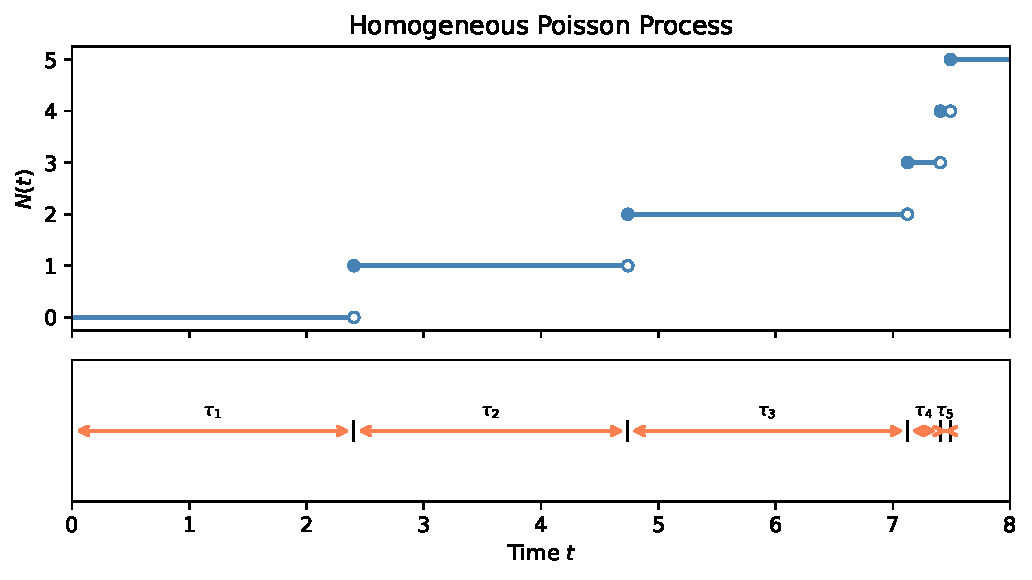
\includegraphics[width=\textwidth]{poisson_process}
    \vspace{0.3em}
    \footnotesize
    \textbf{Uniform order statistics:} Given $N(t)=n$, the arrival times are
    the ordered statistics of $n$ i.i.d.\ $\mathcal{U}(0,t)$ variables.
  \end{columns}
\end{frame}

\begin{frame}[fragile]{Python: Homogeneous Poisson Process}
\begin{lstlisting}[style=python]
import numpy as np

def simulate_poisson(lam, t_max, rng=None):
    """Algorithm PoiPro: simulate Poisson(lambda) on [0, t_max]."""
    if rng is None:
        rng = np.random.default_rng()
    arrivals = []
    t = -np.log(rng.uniform()) / lam          # first inter-arrival
    while t <= t_max:
        arrivals.append(t)
        t += -np.log(rng.uniform()) / lam     # next inter-arrival
    return np.array(arrivals)

# Example: lambda=2, simulate on [0,10]
rng = np.random.default_rng(42)
A = simulate_poisson(lam=2.0, t_max=10.0, rng=rng)
print(f"Number of arrivals: {len(A)}")        # Expected: ~20
print(f"Arrival times: {A[:5].round(3)}")
\end{lstlisting}
\end{frame}

% ── 8.2.2 ────────────────────────────────────────────────
\subsection{8.2.2 Non-homogeneous Poisson Process}

\begin{frame}{8.2.2 Non-homogeneous Poisson Process}
  \begin{block}{Definition 8.2.3}
    $N(t)$ is a \textbf{non-homogeneous Poisson process} with intensity $\lambda(t)$ if:
    \begin{enumerate}
      \item Numbers of points in disjoint intervals are independent.
      \item $N(t,t+h]$ has Poisson distribution with mean $\int_t^{t+h}\lambda(s)\,ds$.
    \end{enumerate}
  \end{block}

  \begin{block}{Thinning Method (Proposition 8.2.4)}
    Let $N_\mathrm{h}(t)$ be homogeneous Poisson with intensity $\lambda_{\max}\ge\lambda(t)$.
    Retain each point $A_i$ independently with probability
    $p(t) = \lambda(t)/\lambda_{\max}$.
    The thinned process is non-homogeneous Poisson with intensity $\lambda(t)$.
  \end{block}

  \begin{center}
    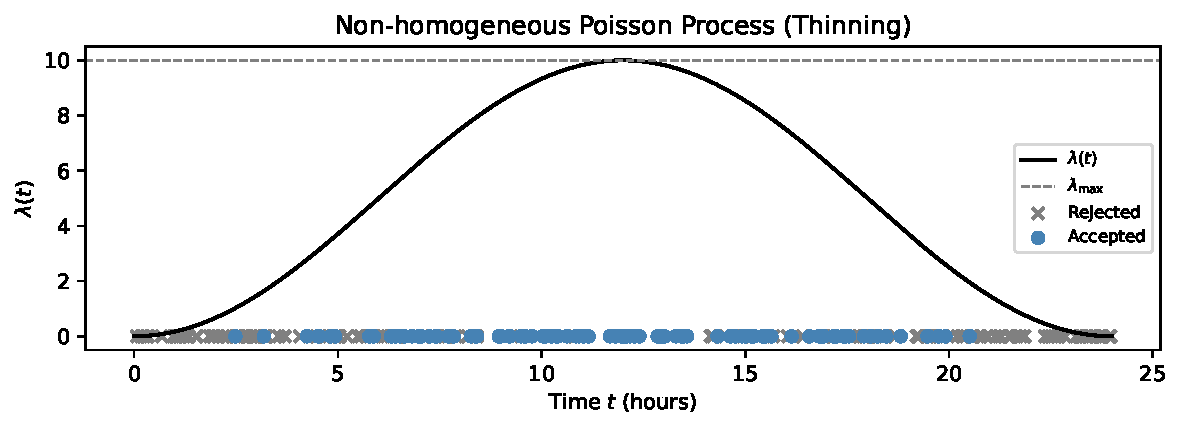
\includegraphics[width=0.72\textwidth]{nhpp_thinning}
  \end{center}
\end{frame}

\begin{frame}[fragile]{Python: NHPP Thinning (Algorithm 75)}
\begin{lstlisting}[style=python]
import numpy as np

def nhpp_thinning(lam_func, lam_max, t_max, rng=None):
    """NH-Poi-thinning: simulate NHPP with intensity lam_func(t)."""
    if rng is None:
        rng = np.random.default_rng()
    A = []
    t = -np.log(rng.uniform()) / lam_max     # Exp(lam_max) jump
    while t <= t_max:
        p = lam_func(t) / lam_max            # acceptance probability
        if rng.uniform() <= p:
            A.append(t)
        t += -np.log(rng.uniform()) / lam_max
    return np.array(A)

# Example: daily arrival pattern lambda(t) = 10*(0.5+0.5*sin(2*pi*t/24))
lam_func = lambda t: 10*(0.5 + 0.5*np.sin(2*np.pi*t/24 - np.pi/2))
rng = np.random.default_rng(7)
A = nhpp_thinning(lam_func, lam_max=10.0, t_max=24.0, rng=rng)
print(f"Arrivals in [0,24]: {len(A)}")
\end{lstlisting}
\end{frame}

% ── 8.2.3 ────────────────────────────────────────────────
\subsection{8.2.3 Poisson Process on General Spaces}

\begin{frame}{8.2.3 Poisson Process on General Spaces}
  \begin{block}{Definition 8.2.6 -- Poisson Point Process on $E\subset\R^d$}
    A point process $N$ on $E$ with intensity measure $\Lambda(\cdot)$ is a
    \textbf{Poisson point process} if:
    \begin{enumerate}
      \item For all disjoint $B_1,\ldots,B_n\in\mathcal{A}$, the counts $N(B_1),\ldots,N(B_n)$ are independent.
      \item $N(B)\sim\mathrm{Poi}(\Lambda(B))$ for all $B\in\mathcal{A}$.
    \end{enumerate}
  \end{block}

  \textbf{Special cases:}
  \begin{itemize}
    \item Homogeneous on $[0,t_{\max}]$: $\Lambda(dt) = \lambda\,dt$.
    \item Non-homogeneous on $[0,t_{\max}]$: $\Lambda(dt) = \lambda(t)\,dt$.
    \item General $E\subset\R^d$: $\Lambda(d\mathbf{x}) = \lambda\,d\mathbf{x}$.
  \end{itemize}

  \begin{block}{Algorithm 77: Finite Intensity $\Lambda(E)<\infty$}
    \begin{enumerate}
      \item Generate $T\sim\mathrm{Poi}(\Lambda(E))$.
      \item Generate $\xi_1,\ldots,\xi_T$ independently from $E$ with distribution $\Lambda(d\mathbf{x})/\Lambda(E)$.
      \item Return points $\xi_1,\ldots,\xi_T$.
    \end{enumerate}
  \end{block}
\end{frame}

\begin{frame}{Poisson Point Process on $[0,3]^2$}
  \begin{columns}
    \column{0.48\textwidth}
    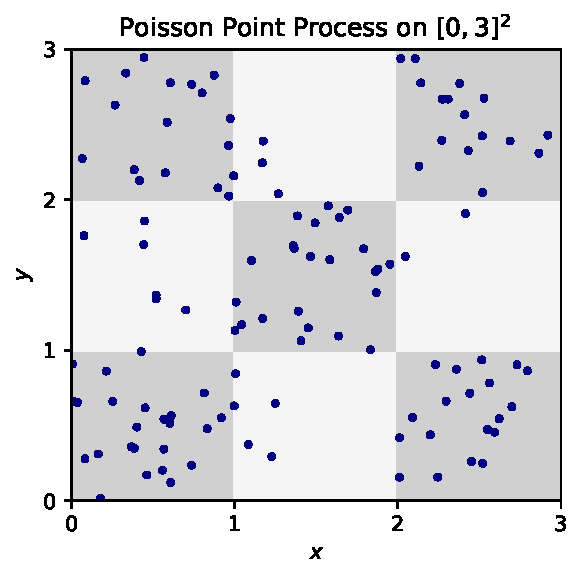
\includegraphics[width=\textwidth]{poisson_2d}

    \column{0.50\textwidth}
    \textbf{Example:} Heterogeneous intensity on $[0,3]^2$:
    \begin{itemize}
      \item Grey cells: intensity $= 20$
      \item White cells: intensity $= 5$
    \end{itemize}
    \vspace{0.5em}
    \textbf{Simulation procedure:}
    \begin{enumerate}
      \item Partition $E = E_1\cup E_2\cup\cdots$
      \item On each $E_j$: simulate $N_j\sim\mathrm{Poi}(\Lambda(E_j))$ points
      \item Points uniform within each $E_j$
    \end{enumerate}
    \vspace{0.3em}
    \textbf{Key property:} If $N_1,N_2$ are independent Poisson processes with intensities $\Lambda_1,\Lambda_2$, then $N_1+N_2$ is Poisson with intensity $\Lambda_1+\Lambda_2$.
  \end{columns}
\end{frame}

% ============================================================
\section{8.3 Birth and Death Processes / Markovian Queues}
% ============================================================

\begin{frame}{8.3 Birth and Death Processes and Markovian Queues}
  \begin{block}{Birth-and-Death Process}
    A continuous-time Markov process $X(t)$ with state space $\{0,1,2,\ldots\}$:
    \begin{itemize}
      \item From state $i$: \emph{birth} (jump to $i+1$) at rate $\lambda_i$.
      \item From state $i$: \emph{death} (jump to $i-1$) at rate $\mu_i$ (with $\mu_0=0$).
    \end{itemize}
    Next event time: $\tau \sim \mathrm{Exp}(\lambda_i + \mu_i)$.\\
    Birth/death selected with probabilities $\lambda_i/(\lambda_i+\mu_i)$ and $\mu_i/(\lambda_i+\mu_i)$.
  \end{block}

  \textbf{Kendall Notation for Queues:} \texttt{A/S/c}
  \begin{itemize}
    \item \texttt{A} = inter-arrival distribution (\texttt{M}=exponential, \texttt{G}=general, \texttt{GI}=i.i.d.)
    \item \texttt{S} = service time distribution
    \item \texttt{c} = number of servers ($c=\infty$ = infinite servers)
  \end{itemize}
\end{frame}

\begin{frame}{M/M/1 Queue}
  \textbf{M/M/1:} Poisson arrivals (rate $\lambda$), exponential service (rate $\mu$), 1 server.

  \begin{block}{Steady-State Mean Queue Length}
    Traffic intensity $\rho = \lambda/\mu < 1$ (stability condition):
    \[
      \bar{l} = \E[L^*] = \frac{\lambda}{\mu-\lambda} = \frac{\rho}{1-\rho}.
    \]
    Stationary distribution: $\pi_i = (1-\rho)\rho^i$, $i=0,1,\ldots$
  \end{block}

  \vspace{0.4em}
  \textbf{Estimation from simulation:}
  \[
    \hat{l}(t_{\max}) = \frac{\int_0^{t_{\max}} L(s)\,ds}{t_{\max}}
    = \frac{1}{t_{\max}}\sum_{j=0}^k y_j(a_{j+1}-a_j)
  \]
  where $a_j$ are event times and $y_j$ the state between events.

  \vspace{0.3em}
  \textbf{Stability:} The system is stable iff $\rho < 1$.  For $\rho \ge 1$, $L(t)\to\infty$.
\end{frame}

\begin{frame}{M/M/1 Simulations}
  \begin{center}
    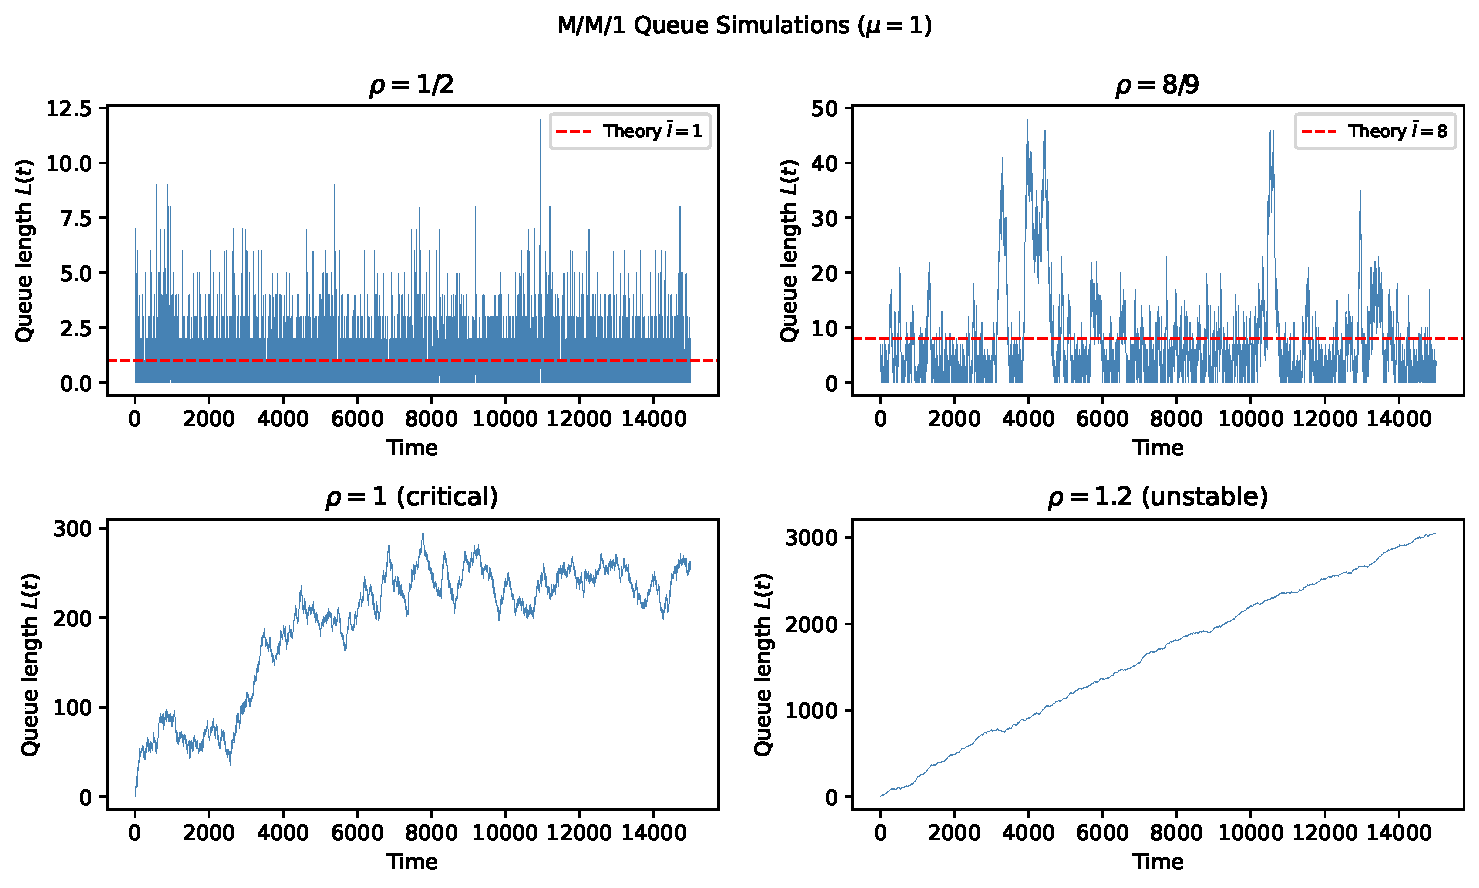
\includegraphics[width=0.85\textwidth]{mm1_simulations}
  \end{center}
  \footnotesize
  Simulations of $L(t)$ for $\mu=1$ and various $\lambda$. (a) $\rho=1/2$: stable, $\bar{l}=1$.
  (b) $\rho=8/9$: stable, $\bar{l}=8$. (c) $\rho=1$: critical, mean diverges.
  (d) $\rho=1.2$: unstable, $L(t)\to\infty$.
\end{frame}

\begin{frame}[fragile]{Python: Birth-and-Death / M/M/1 Simulation}
\begin{lstlisting}[style=python]
import numpy as np

def simulate_mm1(lam, mu, t_max, L0=0, rng=None):
    """Simulate M/M/1 queue via birth-and-death process."""
    if rng is None:
        rng = np.random.default_rng()
    t, L = 0.0, L0
    jump_times, states = [0.0], [L0]
    while t < t_max:
        rate = lam + (mu if L > 0 else 0)
        t += rng.exponential(1/rate)
        if t >= t_max:
            break
        if rng.uniform() < lam / rate:
            L += 1          # arrival (birth)
        else:
            L = max(L-1, 0) # departure (death)
        jump_times.append(t); states.append(L)
    # Compute time-averaged queue length
    ts = np.array(jump_times + [t_max])
    ss = np.array(states + [states[-1]])
    l_hat = np.sum(ss[:-1] * np.diff(ts)) / t_max
    return l_hat, jump_times, states

rng = np.random.default_rng(0)
l_hat, _, _ = simulate_mm1(0.5, 1.0, 1e4, rng=rng)
print(f"Estimated mean: {l_hat:.4f}, Theory: {0.5/0.5:.1f}")
\end{lstlisting}
\end{frame}

% ============================================================
\section{8.4 Basic Concepts of Queueing Theory}
% ============================================================

\begin{frame}{8.4 Basic Concepts of Queueing Theory}
  \begin{columns}
    \column{0.55\textwidth}
    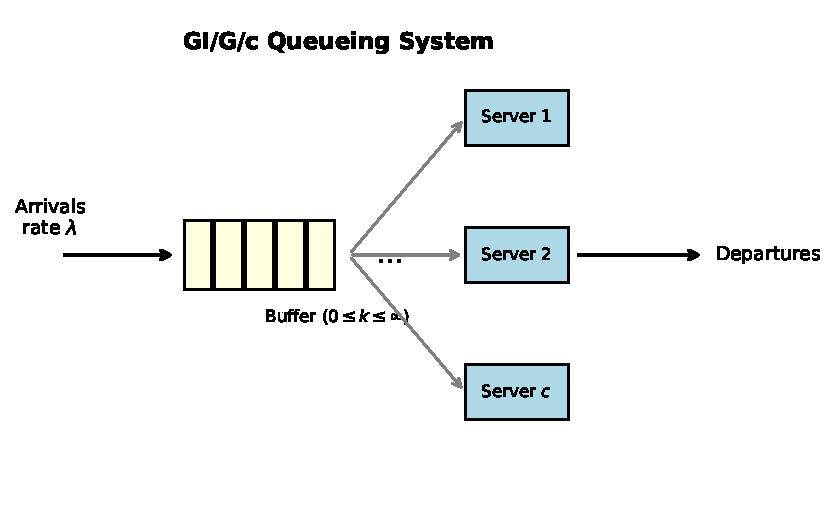
\includegraphics[width=\textwidth]{queue_diagram}

    \column{0.43\textwidth}
    \textbf{System characteristics:}
    \begin{itemize}
      \item $A_i$ = arrival time of $i$-th task
      \item $S_i$ = service time (size) of $i$-th task
      \item $W_i$ = waiting time (before service)
      \item $D_i = A_i + W_i + S_i$ = departure time
      \item $L(t)$ = tasks in system at time $t$
    \end{itemize}

    \vspace{0.4em}
    \textbf{Stability:}\\
    Traffic intensity $\rho = \E[S]/\E[T]$ where $T$ = inter-arrival time.\\
    \emph{Stable} iff $\rho < c$ (for $c$ servers).
  \end{columns}
\end{frame}

\begin{frame}{Little's Law}
  \begin{block}{Little's Law (L = $\lambda$ W)}
    Under mild conditions, for any stable queueing system:
    \[
      \bar{l} = \lambda\,\bar{w},
    \]
    where $\bar{l}$ = steady-state mean number of tasks in system,
    $\lambda$ = arrival rate, $\bar{w}$ = steady-state mean sojourn time.
  \end{block}

  \vspace{0.3em}
  \textbf{Application to M/M/1:}
  \begin{itemize}
    \item $\bar{l} = \rho/(1-\rho)$, $\lambda$ known, so $\bar{w} = \bar{l}/\lambda = 1/(\mu-\lambda)$.
  \end{itemize}

  \begin{center}
    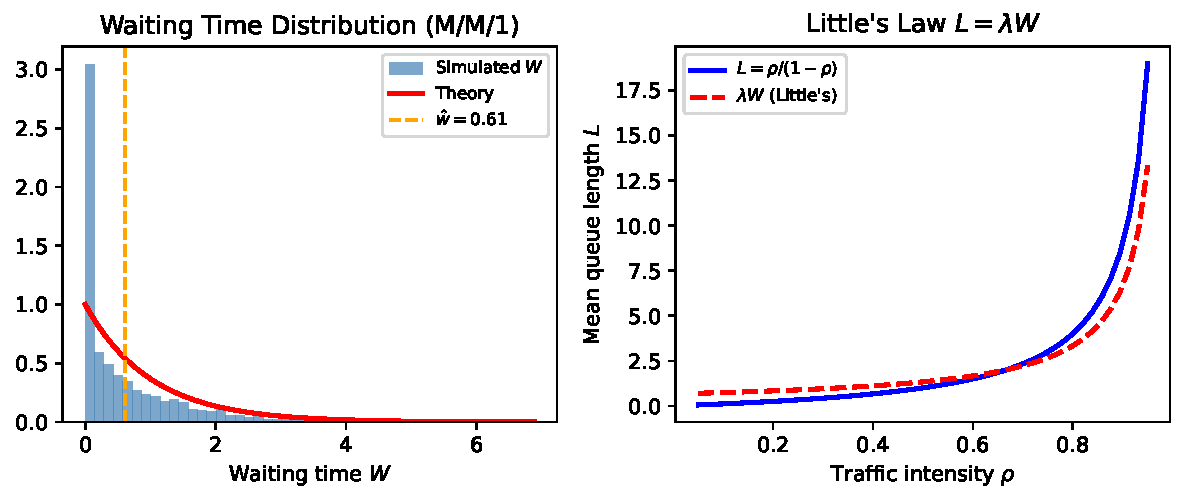
\includegraphics[width=0.60\textwidth]{littles_law}
  \end{center}
\end{frame}

\begin{frame}{GI/G/1 Waiting Time Recursion}
  \begin{block}{Lindley Recursion (Eq.~8.4.1)}
    Under FCFS discipline, $W_1 = 0$ and:
    \[
      W_{i+1} = (W_i + S_i - \tau_{i+1})_+.
    \]
    $W_i$ = waiting time of $i$-th task; $S_i$ = service time; $\tau_{i+1}$ = next inter-arrival.
  \end{block}

  \textbf{Stability:} If $\E[S_1] < \E[\tau_1]$, then $W_i \to W_\infty$ (steady state).\\
  \textbf{Estimate:}
  \[
    \hat{w} = \frac{1}{k}\sum_{i=1}^k W_i.
  \]

  \begin{block}{Pollaczek-Khinchin Formula (M/G/1)}
    When inter-arrivals are $\mathrm{Exp}(\lambda)$:
    \[
      \tilde{w} = \frac{\lambda\E[S_1^2]}{2(1-\lambda\E[S_1])}.
    \]
  \end{block}
\end{frame}

\begin{frame}{$\mathrm{M/G}/\infty$ Systems}
  \textbf{Infinite-server system:} every task is immediately served; no waiting.

  \begin{block}{$\mathrm{M/G}/\infty$ Steady-State Distribution}
    Arrivals: Poisson($\lambda$); service times i.i.d.\ $\sim G$; $\E S_1 = \mu^{-1} < \infty$.
    With $\rho = \lambda/\mu = \lambda\E S$:
    \[
      \Prob(L^* = k) = \frac{\rho^k}{k!}e^{-\rho},\qquad k=0,1,\ldots
    \]
    \[
      \E L^* = \rho = \frac{\lambda}{\mu}, \qquad \text{(Poisson distribution)}
    \]
  \end{block}

  \textbf{Key:} The steady-state distribution depends only on $\rho = \lambda/\mu$, not on the
  specific form of $G$.

  \vspace{0.3em}
  \textbf{Virtual waiting time (workload):}
  \[
    V(t) = \sum_{i=1}^\infty (W_i + S_i - t)_+\,\mathbf{1}(A_i \le t < A_{i+1}).
  \]
\end{frame}

% ============================================================
\section{8.5 Discrete-Event Simulations}
% ============================================================

\begin{frame}{8.5 Discrete-Event Simulations}
  \textbf{Key idea:} System state changes \emph{only at event times} (arrivals, departures).
  Between events, the state is constant.

  \vspace{0.5em}
  \textbf{Core components:}
  \begin{enumerate}
    \item \textbf{Simulation clock} $t$: current simulation time.
    \item \textbf{Event list} (EL): list of pending (time, event\_type) pairs.
    \item \textbf{State variables}: e.g.\ $n$ = number of tasks in system.
    \item \textbf{Output list} JS: records $(t(i), n(i))$ pairs at each event.
  \end{enumerate}

  \vspace{0.5em}
  \textbf{On-Off Process as simplest example:}
  \begin{itemize}
    \item State alternates between 0 (off) and 1 (on).
    \item On-times $\sim F_{\mathrm{on}}$, off-times $\sim F_{\mathrm{off}}$.
    \item Steady-state probability of being on:
    \[
      p = \frac{\E T^{\mathrm{on}}}{\E T^{\mathrm{on}} + \E T^{\mathrm{off}}}.
    \]
  \end{itemize}
\end{frame}

\begin{frame}{On-Off Process}
  \begin{center}
    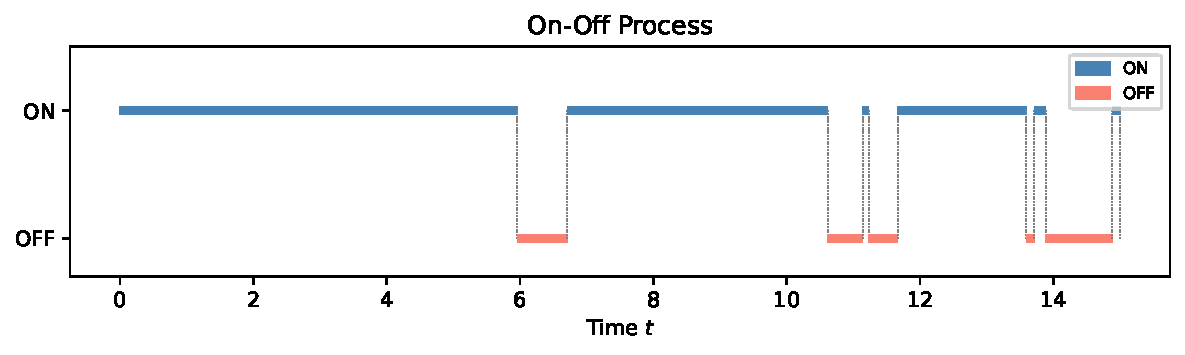
\includegraphics[width=0.85\textwidth]{onoff_process}
  \end{center}

  \begin{block}{Estimator of $p$}
    \[
      \hat{p}(t_{\max}) = \frac{1}{t_{\max}}\int_0^{t_{\max}} K(s)\,ds,
    \]
    where $K(t)\in\{0,1\}$ is the current state. This estimator is strongly consistent.
  \end{block}
\end{frame}

\begin{frame}[fragile]{Python: On-Off Discrete-Event Simulation}
\begin{lstlisting}[style=python]
import numpy as np

def simulate_onoff(lam_on, lam_off, t_max, rng=None):
    """Discrete-event simulation of on-off process."""
    if rng is None:
        rng = np.random.default_rng()
    t = 0.0; state = 1  # start in ON state
    integral = 0.0      # accumulate time in ON state
    events = [(0.0, 1)]
    while t < t_max:
        # Time until next switch
        if state == 1:
            dt = rng.exponential(1/lam_on)
        else:
            dt = rng.exponential(1/lam_off)
        new_t = min(t + dt, t_max)
        integral += state * (new_t - t)
        t = new_t
        if t < t_max:
            state = 1 - state
        events.append((t, state))
    p_hat = integral / t_max
    return p_hat, events

# Example: E[T^on]=3, E[T^off]=1, p = 3/4
rng = np.random.default_rng(5)
p_hat, _ = simulate_onoff(1/3, 1.0, t_max=10000, rng=rng)
print(f"p_hat = {p_hat:.4f}, theory = 0.75")
\end{lstlisting}
\end{frame}

\subsection{8.5.1 GI/G/c Queue}

\begin{frame}{GI/G/c Queue}
  \textbf{Discrete-event simulation of a $c$-server queue with general distributions.}

  \begin{block}{Single-Server GI/G/1: Algorithm 81}
    State: arrival time $t_A$, departure time $t_D$, queue size $n$.
    \begin{enumerate}
      \item Initialize: $t_A \sim F$, EL = $[t_A, \emptyset]$.
      \item \textbf{While} $t_A < t_{\max}$, process events:
        \begin{itemize}
          \item \textbf{Arrival} (EL empty): service $S\sim G$, $t_D = t_A + S$; next arrival.
          \item \textbf{Both in EL}: if $t_A < t_D$ (arrival first): $n\mathrel{+}= 1$.
          \item Otherwise (departure first): $n\mathrel{-}= 1$; if $n>0$, new service.
        \end{itemize}
    \end{enumerate}
  \end{block}

  \begin{block}{GI/G/c Workload Recursion}
    Vector $\mathbf{V}_i = (V_{i,1},\ldots,V_{i,c})$ of server workloads, sorted:
    \[
      \mathbf{V}_{i+1} = \mathrm{sort}\bigl((V_{i,1}+S_i-\tau_{i+1})_+,\,
                                              (V_{i,2}-\tau_{i+1})_+,\,\ldots,\,
                                              (V_{i,c}-\tau_{i+1})_+\bigr).
    \]
    Waiting time of $i$-th task: $W_i = V_{i,1}$ (smallest workload).
    Stable iff $\rho = \E S/\E\tau < c$.
  \end{block}
\end{frame}

\begin{frame}{GI/G/1 Queue Path}
  \begin{center}
    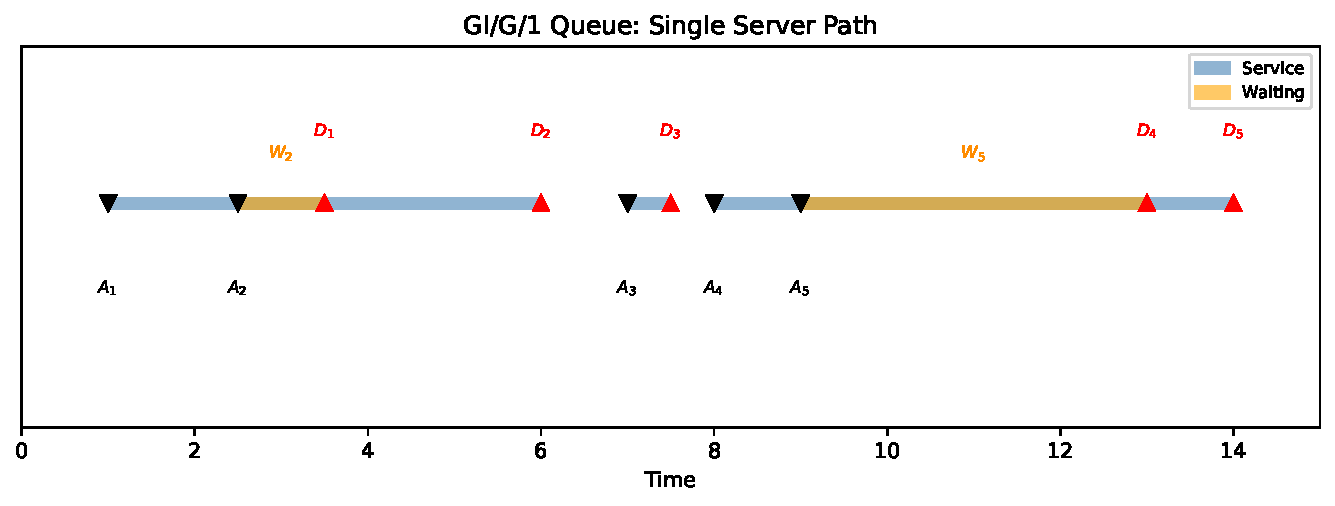
\includegraphics[width=0.85\textwidth]{gig1_path}
  \end{center}
  \footnotesize
  Example path: arrivals (down arrows), service intervals (blue), waiting times (orange), departures (up arrows).
\end{frame}

\begin{frame}[fragile]{Python: GI/G/1 Waiting Times}
\begin{lstlisting}[style=python]
import numpy as np

def gig1_waiting_times(n_tasks, F_interarr, G_service, rng=None):
    """Sample waiting times W_1,...,W_n for GI/G/1 (FCFS)."""
    if rng is None:
        rng = np.random.default_rng()
    tau = F_interarr(n_tasks, rng)   # inter-arrival times
    S   = G_service(n_tasks, rng)    # service times
    W = np.zeros(n_tasks)
    for i in range(1, n_tasks):
        W[i] = max(W[i-1] + S[i-1] - tau[i], 0)
    return W

# M/M/1 example: lambda=0.5, mu=1
rng = np.random.default_rng(0)
F = lambda n, r: r.exponential(2.0, n)    # Exp(1/2), mean=2
G = lambda n, r: r.exponential(1.0, n)    # Exp(1), mean=1
W = gig1_waiting_times(10000, F, G, rng)
w_hat = np.mean(W)
# Theory: w = lambda*E[S^2]/(2*(1-rho)) with Exp service: E[S^2]=2
rho = 0.5
w_theory = rho/(1-rho)/1.0   # for M/M/1: w = rho/(mu*(1-rho))
print(f"w_hat = {w_hat:.4f}, theory = {w_theory:.4f}")
\end{lstlisting}
\end{frame}

% ============================================================
\section{8.6 Slotted ALOHA}
% ============================================================

\begin{frame}{8.6 Slotted ALOHA and Random Access Protocols}
  \textbf{Setup:} Shared transmission channel; time divided into slots.

  \begin{columns}
    \column{0.55\textwidth}
    \textbf{Packet dynamics:}
    \begin{itemize}
      \item $X_n$ = packets waiting at start of slot $n$.
      \item $A_n\sim\mathrm{Poi}(\lambda)$ = new arrivals in slot $n$.
      \item $Z_n$ = transmissions in slot $n$.
      \item Successful if $Z_n = 1$ (no collision).
    \end{itemize}

    \begin{block}{Queue Update (8.6.1)}
      \[
        X_{n+1} = X_n + A_n - \mathbf{1}(Z_n=1), \quad n=0,1,\ldots
      \]
    \end{block}

    \column{0.43\textwidth}
    \textbf{Retransmission strategies:}
    \begin{itemize}
      \item \textbf{Slotted ALOHA}: retry with fixed prob.\ $h$
      \item \textbf{Exp.\ Back-off}: $h_i = 2^{-i}$
      \item \textbf{Ethernet}: $h_i = 2^{-i}$ up to $K$ attempts
    \end{itemize}

    \begin{block}{Conditional Distribution}
      $Z_n \mid X_n = k$: $A_n + Y_n$, $Y_n\sim\mathrm{Bin}(k,h)$
    \end{block}
  \end{columns}
\end{frame}

\begin{frame}{Slotted ALOHA: Instability}
  \begin{center}
    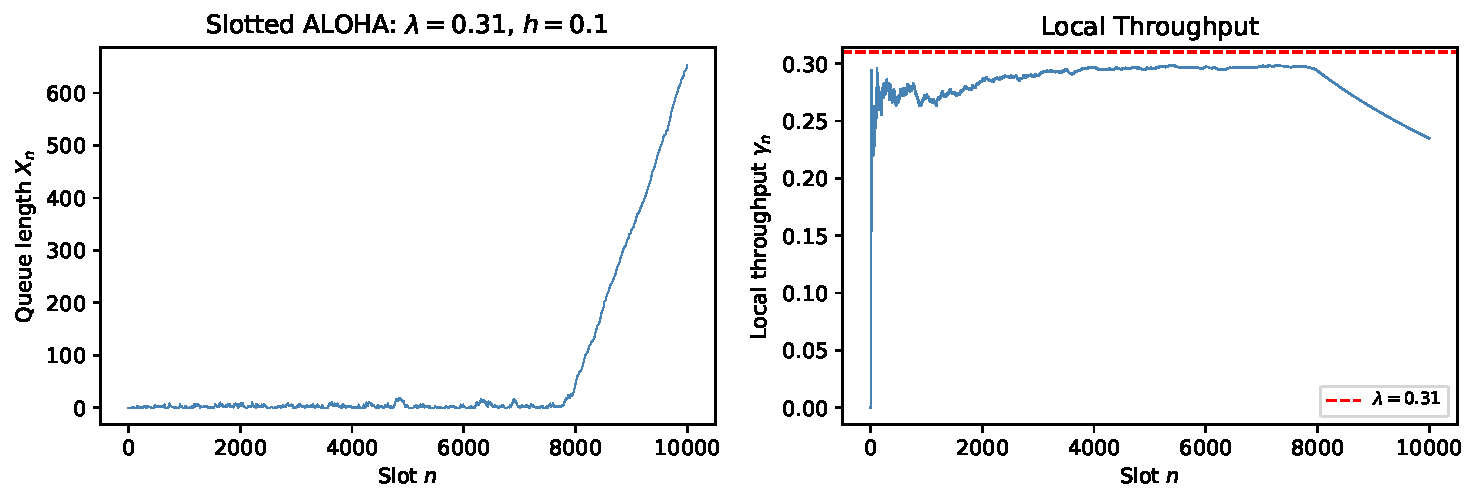
\includegraphics[width=0.85\textwidth]{slotted_aloha}
  \end{center}

  \begin{block}{Conditional Drift}
    \[
      \E[X_{n+1}-X_n \mid X_n=k]
      = \lambda - e^{-\lambda}\,kh(1-h)^{k-1} - \lambda e^{-\lambda}(1-h)^k.
    \]
    As $k\to\infty$: drift $\to\lambda > 0$.
    \textbf{The queue grows without bound} $\Rightarrow$ Slotted ALOHA is inherently unstable!
  \end{block}
\end{frame}

\begin{frame}[fragile]{Python: Slotted ALOHA Simulation}
\begin{lstlisting}[style=python]
import numpy as np

def simulate_aloha(lam, h, n_slots, rng=None):
    """Simulate Slotted ALOHA with Poisson arrivals."""
    if rng is None:
        rng = np.random.default_rng()
    X = 0; Xs = [0]; successes = 0; throughputs = [0.0]
    for n in range(1, n_slots+1):
        A = rng.poisson(lam)                       # new arrivals
        Y = rng.binomial(X, h) if X > 0 else 0    # retransmissions
        transmitting = A + Y
        success = int(transmitting == 1)
        successes += success
        X = max(X + A - success, 0)
        Xs.append(X)
        throughputs.append(successes / n)
    return np.array(Xs), np.array(throughputs)

# Critical region: lambda=0.31, h=0.1
rng = np.random.default_rng(11)
Xs, gammas = simulate_aloha(0.31, 0.1, 10000, rng)
print(f"Final queue: {Xs[-1]}, Final throughput: {gammas[-1]:.3f}")
\end{lstlisting}
\end{frame}

% ============================================================
\section{8.7 Ergodically Stable Processes}
% ============================================================

\begin{frame}{8.7 Ergodically Stable Processes}
  \begin{block}{Stationary Process}
    $X^*(t)$ is \textbf{stationary} if the joint distribution of
    $(X^*(t+h_1),\ldots,X^*(t+h_d))$ does not depend on $t$.
    \begin{itemize}
      \item Marginal distributions: $\E[X^*(t)]$ and $\Var[X^*(t)]$ are constant.
      \item Covariance function: $R(h) = \mathrm{Cov}(X^*(t),X^*(t+h))$ depends only on $h$.
    \end{itemize}
  \end{block}

  \begin{block}{Ergodic Process}
    A stationary process $X^*(t)$ is \textbf{ergodic} if for any function $g$:
    \[
      \lim_{t\to\infty}\frac{1}{t}\int_0^t g(X^*(h_1+s),\ldots,X^*(h_d+s))\,ds
      = \E[g(X^*(h_1),\ldots,X^*(h_d))].
      \tag{8.7.2}
    \]
    In particular ($d=1$):
    \[
      \lim_{t\to\infty}\frac{1}{t}\int_0^t X^*(s)\,ds = \E[X^*(0)].
    \]
  \end{block}
\end{frame}

\begin{frame}{Ergodically Stable Processes}
  \begin{block}{Definition: Ergodically Stable}
    $X(t)$ is \textbf{ergodically stable} if there exists a stationary ergodic process
    $X^*(t)$ such that, with probability 1:
    \[
      \lim_{t\to\infty}\frac{1}{t}\int_0^t g(X(h_1+s),\ldots,X(h_d+s))\,ds
      = \E[g(X^*(h_1),\ldots,X^*(h_d))].
    \]
    Key property: time averages converge to ensemble averages, regardless of initial state.
  \end{block}

  \begin{block}{Practical Implication}
    \[
      \lim_{t\to\infty}\frac{1}{t}\int_0^t X(s)\,ds = \E[X^*(0)] = I, \quad\text{a.s.}
    \]
    So the \emph{time average} $\hat{X}(t) = \frac{1}{t}\int_0^t X(s)\,ds$ is a
    consistent estimator of $I = \E[X^*]$.
  \end{block}
\end{frame}

\begin{frame}{Central Limit Theorem for Ergodic Processes}
  \begin{block}{CLT (8.7.4)}
    For an ergodic process satisfying mild conditions:
    \[
      \sqrt{t}\bigl(\hat{X}^*(t) - \E[X^*(0)]\bigr)
      \xrightarrow{\mathcal{D}} \mathcal{N}(0, \varsigma^2),
    \]
    where $\varsigma^2$ is the \textbf{asymptotic variance} (TAVC).
  \end{block}

  \begin{block}{Fundamental Error--Precision Relationship}
    \[
      b = z_{1-\alpha/2}\,\frac{\varsigma}{\sqrt{t}},
    \]
    $b$ = confidence interval half-width at level $1-\alpha$; $z_{1-\alpha/2}$ = normal quantile.
  \end{block}

  \textbf{Confidence interval:}
  \[
    \hat{X}^*(t) \pm \frac{z_{1-\alpha/2}\,\varsigma}{\sqrt{t}}.
  \]
\end{frame}

\subsection{8.7.1 Asymptotic Variance Formula}

\begin{frame}{8.7.1 Asymptotic Variance (TAVC)}
  \begin{block}{Lemma 8.7.5 -- TAVC Formula}
    If $\int_0^\infty |R(v)|\,dv < \infty$ and $\int_0^\infty R(s)\,ds \ne 0$, then:
    \[
      \Var\!\left(\int_0^t X^*(s)\,ds\right) \sim 2t\int_0^\infty R(v)\,dv, \quad t\to\infty.
    \]
    Therefore:
    \[
      \varsigma^2 = 2\int_0^\infty R(v)\,dv.
      \tag{8.7.9}
    \]
    $R(h) = \mathrm{Cov}(X^*(t), X^*(t+h))$ = covariance function of the stationary process.
  \end{block}

  \begin{center}
    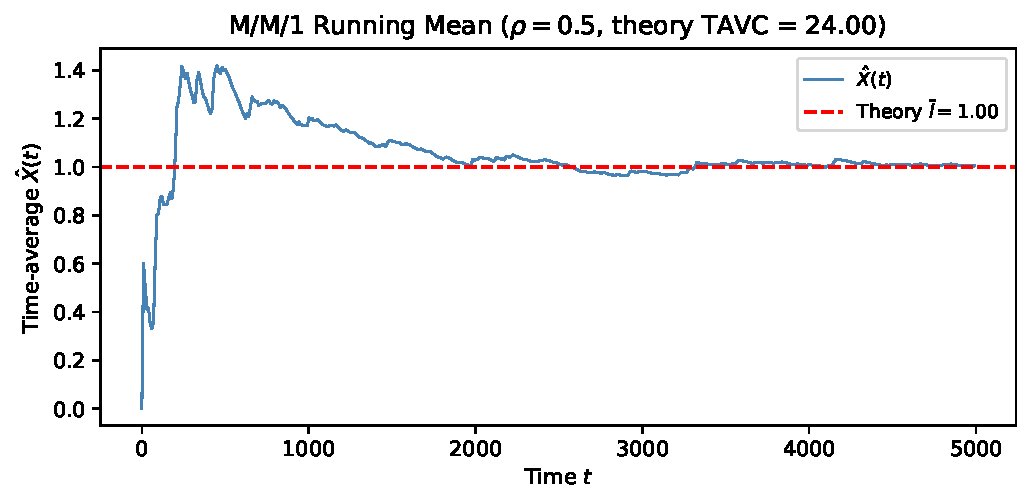
\includegraphics[width=0.55\textwidth]{tavc_illustration}
  \end{center}
\end{frame}

\begin{frame}{TAVC for the On-Off Process}
  \begin{block}{Asymptotic Variance of On-Off Process (8.7.11)}
    \[
      \varsigma^2 = \frac{(\E T^{\mathrm{on}})^2\,\Var T^{\mathrm{off}}
                        + (\E T^{\mathrm{off}})^2\,\Var T^{\mathrm{on}}}
                        {(\E T^{\mathrm{on}} + \E T^{\mathrm{off}})^3}.
    \]
    \textbf{Special case} $T^{\mathrm{on}}\sim\mathrm{Exp}(\lambda)$, $T^{\mathrm{off}}\sim\mathrm{Exp}(\mu)$:
    \[
      \varsigma^2 = 2\,\frac{\lambda\mu}{(\lambda+\mu)^3}
                 = \frac{2\rho}{\mu(1+\rho)^3}, \quad \rho = \lambda/\mu.
    \]
  \end{block}

  \textbf{M/M/1 Queue TAVC (8.9.3):}
  \[
    \varsigma_L^2 = \frac{2\rho(1+\rho)}{\mu(1-\rho)^4}.
  \]
  This grows like $(1-\rho)^{-4}$ as $\rho\nearrow 1$ (heavy traffic).
\end{frame}

\subsection{8.7.2 TAVC for Other Systems}

\begin{frame}{8.7.2 TAVC for Other Systems}
  \begin{block}{Finite B\&D Process (Whitt--Burman Formula, 8.7.14)}
    For $Y(t) = f(X(t))$ with B\&D process $X(t)$, stationary mean $I_f$:
    \[
      \varsigma_f^2 = 2\sum_{j=0}^{n-1}\frac{1}{\lambda_j\pi_j}
                       \left[\sum_{i=0}^{j}(f(i)-I_f)\pi_i\right]^2.
    \]
    Stationary distribution: $\pi_i = \pi_0\,\frac{\lambda_0\cdots\lambda_{i-1}}{\mu_1\cdots\mu_i}$.
  \end{block}

  \begin{block}{M/M/$n$ Queue TAVC}
    With $\rho=\lambda/\mu$, $E_n(\rho) = \sum_{j=0}^n \rho^j/j!$:
    \[
      \varsigma^2 = \frac{2}{\lambda}\sum_{j=0}^n \frac{1}{\rho^j/j!}\cdot
                   \frac{\left(\rho(E_{n-1}(\rho) - E_{j-1}(\rho))\right)^2}{E_n(\rho)}.
    \]
  \end{block}

  \begin{center}
    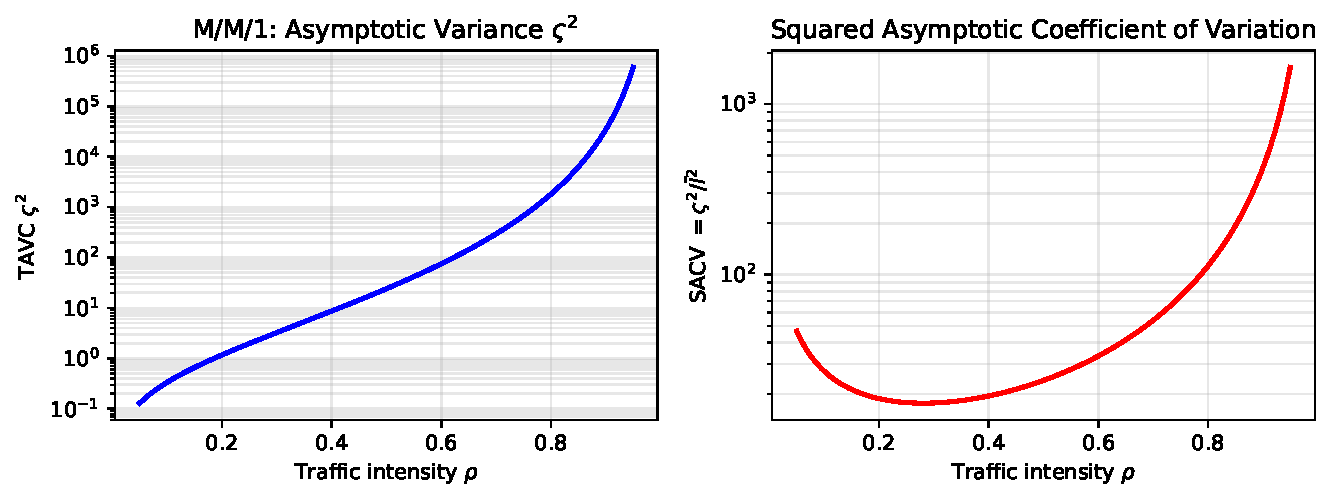
\includegraphics[width=0.55\textwidth]{tavc_vs_rho}
  \end{center}
\end{frame}

% ============================================================
\section{8.8 Regenerative Processes}
% ============================================================

\begin{frame}{8.8 Regenerative Processes}
  \begin{block}{Definition 8.8.1}
    $X(t)$ is \textbf{regenerative} if there exist random times
    $0 =: T_0 \le T_1 < T_2 < \cdots$ such that:
    \begin{itemize}
      \item Pairs $(Z_i, C_i)$ are independent for $i\ge 0$ and i.i.d.\ for $i\ge 1$, where
        $C_i = T_{i+1}-T_i$ (cycle length) and $Z_i = \int_{T_i}^{T_{i+1}} X(s)\,ds$ (integral over cycle).
    \end{itemize}
    The process \emph{restarts} probabilistically at each $T_i$.
  \end{block}

  \textbf{Examples:}
  \begin{itemize}
    \item \textbf{On-off process}: regenerates when entering state 1 (on).
    \item \textbf{M/M/1 queue}: regenerates at times when $L(t-)=0$ and a new arrival occurs.
    \item \textbf{GI/G/1 queue}: regenerates at start of busy periods.
  \end{itemize}

  \begin{center}
    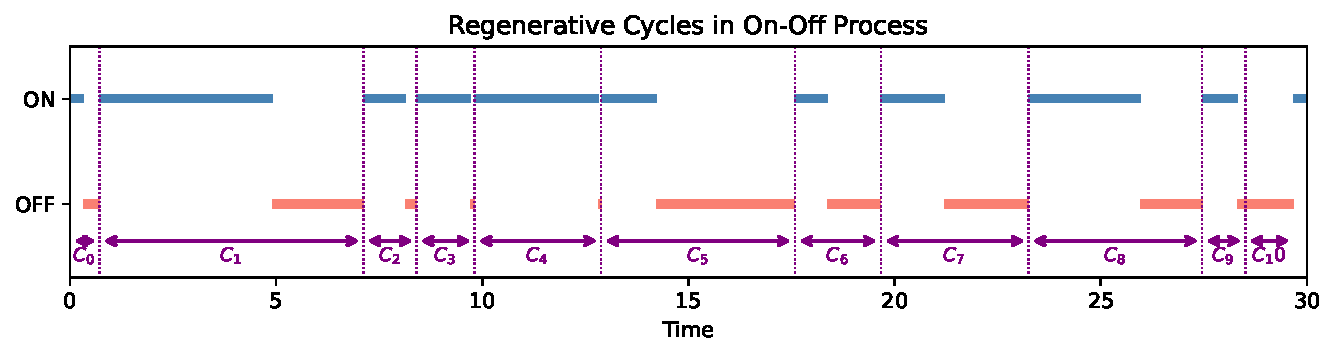
\includegraphics[width=0.75\textwidth]{regenerative_cycles}
  \end{center}
\end{frame}

\begin{frame}{Renewal-Reward Theorem}
  \begin{block}{Proposition 8.8.2 (Renewal Reward)}
    If $\E C_1 < \infty$ and $\E|Z_1| < \infty$, then with probability 1:
    \[
      \hat{X}(t) \to I = \frac{\E\int_{T_1}^{T_2} X(s)\,ds}{\E C_1}, \quad t\to\infty.
      \tag{8.8.1}
    \]
    If additionally $\E C_1^2 < \infty$ and $\Var Z_1 < \infty$, then:
    \[
      \sqrt{t}(\hat{X}(t) - I) \xrightarrow{\mathcal{D}} \mathcal{N}(0,\varsigma_A^2),
    \]
    where $\varsigma_A^2 = \E\zeta_1^2/\E C_1$, $\zeta_k = Z_k - I\,C_k$.
  \end{block}

  \begin{block}{Regenerative Estimator}
    Using $k$ complete cycles after $T_1$:
    \[
      \hat{I}_k = \frac{Z_1+\cdots+Z_k}{C_1+\cdots+C_k}, \qquad
      \varsigma_B^2 = \frac{\E\zeta_1^2}{(\E C_1)^2}.
      \tag{8.8.6, 8.8.7}
    \]
    $\hat{I}_k$ is \textbf{unbiased} if the first cycle is discarded. Asymptotically both $\hat{X}(t)$ and $\hat{I}_k$ have the same CI width.
  \end{block}
\end{frame}

\begin{frame}{On-Off Process: Estimator Comparison}
  \begin{columns}
    \column{0.52\textwidth}
    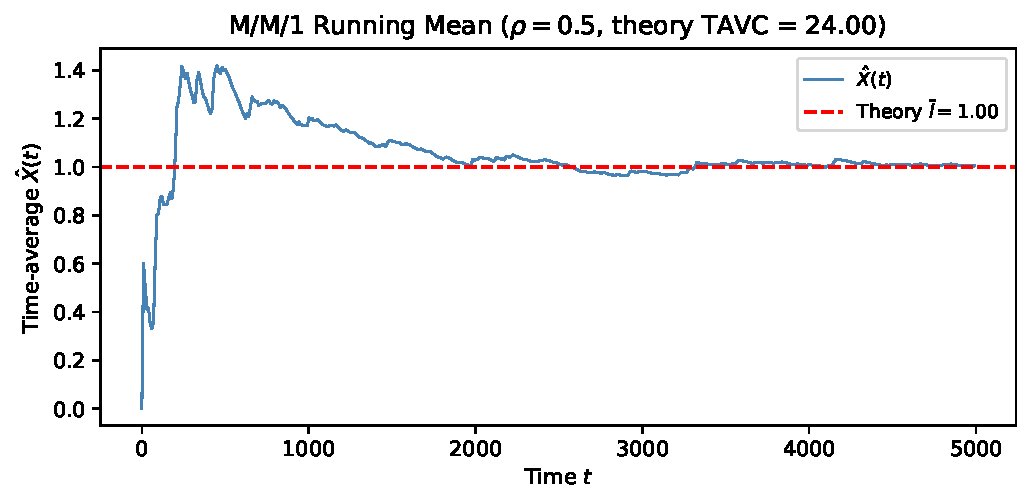
\includegraphics[width=\textwidth]{tavc_illustration}

    \column{0.46\textwidth}
    \textbf{Example (Table 8.2):}\\[0.3em]
    True $p = 3/4$. Two options:
    \begin{itemize}
      \item Opt.~1: $T^{\mathrm{on}}\sim\mathrm{Exp}(1/3)$, $T^{\mathrm{off}}\sim\mathrm{Exp}(1)$
      \item Opt.~2: $T^{\mathrm{on}}\sim\mathrm{Par}(2.5,1.8)$, $T^{\mathrm{off}}\sim\mathrm{Gamma}(2,1/2)$
    \end{itemize}

    \vspace{0.3em}
    \begin{tabular}{lcc}
      \toprule
       & Opt.~1 & Opt.~2 \\
      \midrule
      $\hat{X}(t_{\max})$ & 0.727 & 0.739 \\
      $\hat{I}_k$ & 0.725 & 0.739 \\
      \bottomrule
    \end{tabular}

    \vspace{0.4em}
    \footnotesize
    Both converge to true $p=0.75$. $\hat{I}_k$ is unbiased (discards first cycle).
  \end{columns}
\end{frame}

\begin{frame}[fragile]{Python: Regenerative Estimation}
\begin{lstlisting}[style=python]
import numpy as np

def regenerative_onoff(lam_on, lam_off, n_cycles, rng=None):
    """Regenerative estimator for on-off process (Exp distributions)."""
    if rng is None:
        rng = np.random.default_rng()
    Zs, Cs = [], []
    for _ in range(n_cycles):
        T_on  = rng.exponential(1/lam_on)
        T_off = rng.exponential(1/lam_off)
        C = T_on + T_off
        Z = T_on           # integral of state=1 over cycle
        Zs.append(Z); Cs.append(C)
    Zs, Cs = np.array(Zs), np.array(Cs)
    # Discard first cycle (non-delayed start)
    Z1, C1 = Zs[1:], Cs[1:]
    I_hat = np.sum(Z1) / np.sum(C1)   # regenerative estimator
    # TAVC estimate
    I_cycle = np.sum(Z1) / np.sum(C1)
    zeta = Z1 - I_cycle * C1
    sigma2_B = np.var(zeta, ddof=1) / (np.mean(C1)**2)
    return I_hat, sigma2_B

rng = np.random.default_rng(3)
I_hat, s2 = regenerative_onoff(1/3, 1.0, 300, rng)
print(f"I_hat = {I_hat:.4f}, TAVC = {s2:.4f}")
print(f"95% CI: ({I_hat - 1.96*np.sqrt(s2/300):.4f}, {I_hat + 1.96*np.sqrt(s2/300):.4f})")
\end{lstlisting}
\end{frame}

% ============================================================
\section{8.9 Error Analysis of M/M/1 and M/G/$\infty$}
% ============================================================

\begin{frame}{8.9 Error Analysis of M/M/1 Queue}
  \begin{block}{Steady-State Mean (8.9.2)}
    \[
      \bar{l} = \E[L^*(0)] = \frac{\rho}{1-\rho}, \qquad \rho = \lambda/\mu < 1.
    \]
    Asymptotic variance (8.9.3):
    \[
      \varsigma_L^2 = \frac{2\rho(1+\rho)}{\mu(1-\rho)^4}.
    \]
  \end{block}

  \begin{block}{Required Simulation Length}
    SACV $= \varsigma^2/I^2$. For $b=0.1I$ (10\% relative error), $\alpha=0.05$:
    \[
      t_{\max} = 400 \cdot \mathrm{SACV}, \qquad
      \mathrm{SACV} = \frac{2(1+\rho)}{\mu\rho(1-\rho)^2}.
    \]
  \end{block}

  \textbf{Numerical example:}
  \begin{itemize}
    \item $\rho=1/2$: SACV $= 24$, $t_{\max} = 9600$. Sim.\ gave $\hat{l}=0.9822$ vs $\bar{l}=1$.
    \item $\rho=8/9$: SACV $= 344.25$, $t_{\max} = 1.377\times 10^5$. Sim.\ gave $\hat{l}=6.67$ vs $\bar{l}=8$.
  \end{itemize}
\end{frame}

\begin{frame}{M/M/1 TAVC and Run Length vs.\ $\rho$}
  \begin{center}
    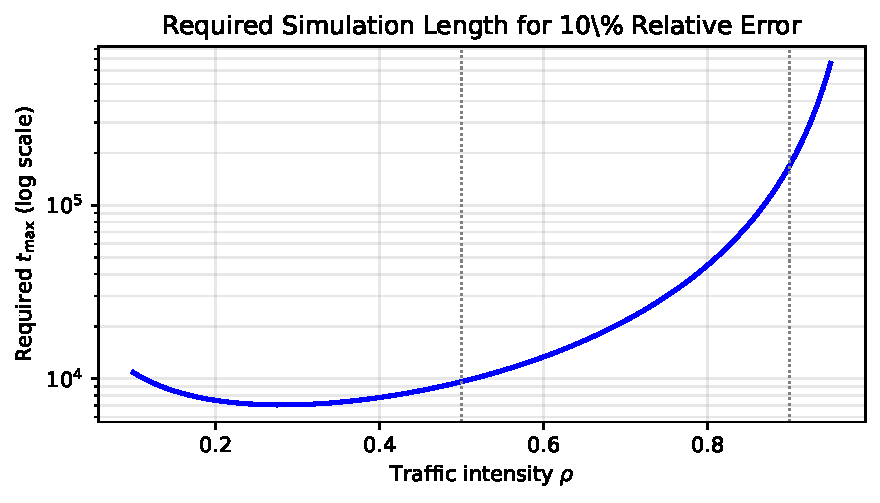
\includegraphics[width=0.82\textwidth]{run_length_vs_rho}
  \end{center}
  \begin{itemize}
    \item Required run length grows as $(1-\rho)^{-2}$ for \emph{relative} error.
    \item Grows as $(1-\rho)^{-4}$ for \emph{absolute} error.
    \item E.g.\ $\rho=0.95$ vs $\rho=0.5$: factor 100$\times$ (relative), 10000$\times$ (absolute)!
  \end{itemize}
\end{frame}

\begin{frame}{8.9 Error Analysis of $\mathrm{M/G}/\infty$ Systems}
  \begin{block}{$\mathrm{M/G}/\infty$ Covariance and TAVC (8.9.4)}
    \[
      R(t) = \lambda\int_t^\infty(1-G(v))\,dv, \qquad
      \varsigma^2 = 2\int_0^\infty R(t)\,dt = 2\lambda\int_0^\infty\int_t^\infty(1-G(v))\,dv\,dt.
    \]
    \textbf{Special case} $G=\mathrm{Exp}(\mu)$: $\varsigma^2 = 2\lambda/\mu = 2\rho$.
  \end{block}

  \textbf{Sensitivity to service distribution:}
  \begin{itemize}
    \item Light-tailed $G$ (Exp): $\varsigma^2 < \infty$, fast convergence.
    \item Heavy-tailed $G = \mathrm{Par}(\alpha)$:
      \begin{itemize}
        \item $\alpha > 2$: finite variance, $\varsigma^2 < \infty$.
        \item $1 < \alpha \le 2$: infinite variance, $\varsigma^2 = \infty$; CLT may fail.
      \end{itemize}
  \end{itemize}

  \begin{center}
    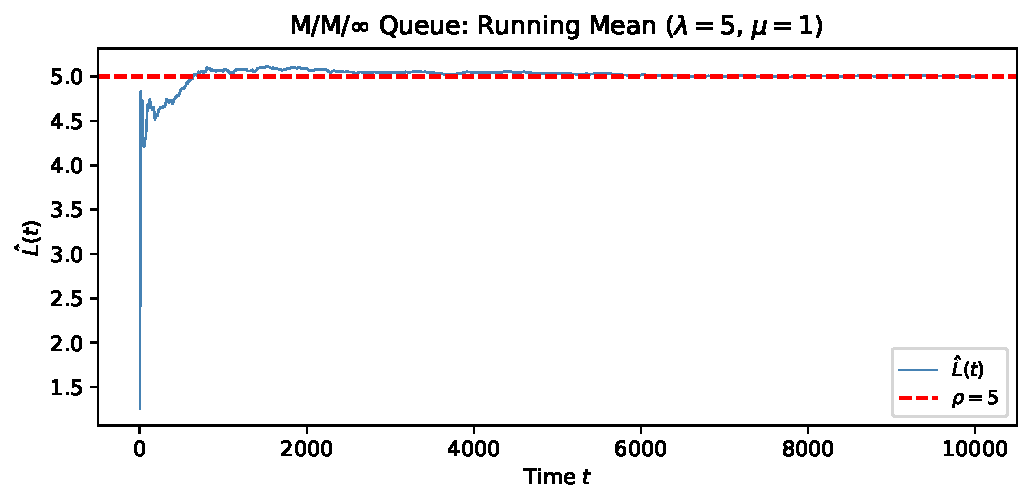
\includegraphics[width=0.60\textwidth]{mginf_estimates}
  \end{center}
\end{frame}

\begin{frame}[fragile]{Python: $\mathrm{M/G}/\infty$ Simulation}
\begin{lstlisting}[style=python]
import numpy as np

def simulate_mginf(lam, G_sample, t_max, rng=None):
    """Simulate M/G/inf queue and estimate steady-state mean."""
    if rng is None:
        rng = np.random.default_rng()
    # Generate arrivals (Poisson process)
    arrivals = []
    t = rng.exponential(1/lam)
    while t < t_max:
        arrivals.append(t); t += rng.exponential(1/lam)
    arrivals = np.array(arrivals)
    service  = G_sample(len(arrivals), rng)
    departures = arrivals + service
    # Estimate: l_hat = integral of L(t) / t_max
    # Using formula (8.9.5): sum of min(t_max, D_i) - A_i
    L_integral = np.sum(np.minimum(departures, t_max) - arrivals)
    l_hat = L_integral / t_max
    return l_hat

rng = np.random.default_rng(99)
# Exponential service: E[S]=1, rho=5
l_hat = simulate_mginf(5.0, lambda n, r: r.exponential(1.0, n), 1e4, rng)
print(f"M/M/inf estimate: {l_hat:.4f}, theory rho=5.0")
# Pareto service (heavy-tailed)
l_hat2 = simulate_mginf(5.0, lambda n, r: 2.2*(r.pareto(3.2, n)+1), 1e4, rng)
print(f"M/Par/inf estimate: {l_hat2:.4f}")
\end{lstlisting}
\end{frame}

% ============================================================
\section{8.10 Bibliographical Notes}
% ============================================================

\begin{frame}{8.10 Bibliographical Notes}
  \textbf{Key references:}
  \begin{itemize}
    \item \textbf{Poisson processes:} Billingsley~[14] for theoretical foundations.
    \item \textbf{Queueing theory:} Ross~[175--177]; Asmussen~[7]; Kleinrock~[117,118].
    \item \textbf{TAVC / SACV:} Kopocinski~[111]; Whitt~[213] (B\&D formula); Reynolds~[173].
    \item \textbf{Regenerative processes:} Asmussen \& Glynn~[8]; Thorisson~[199].
    \item \textbf{Discrete-event simulation:} Law~[130]; Bratley et al.~[22].
    \item \textbf{Random access protocols:} Bertsekas \& Gallager~[13] (ALOHA).
  \end{itemize}

  \vspace{0.5em}
  \textbf{Summary of Chapter 8 algorithms:}
  \begin{itemize}
    \item Alg.~73: \texttt{PoiPro}($\lambda$) -- homogeneous Poisson
    \item Alg.~74: \texttt{PoiProSorted}($\lambda$) -- order-statistics method
    \item Alg.~75: \texttt{NH-Poi-thinning}($\lambda(t)$) -- NHPP via thinning
    \item Alg.~76: \texttt{NH-Poi}($\lambda(t)$) -- NHPP via inverse CDF
    \item Alg.~77: Poisson process on $E$ -- general spaces
    \item Alg.~78: \texttt{BD} -- birth-and-death process
    \item Alg.~79: Repairman problem
    \item Alg.~80--81: Discrete-event simulation of GI/G/c queue
    \item Alg.~82: $\mathrm{M/G}/\infty$ simulation
  \end{itemize}
\end{frame}

% ── Summary ──────────────────────────────────────────────
\begin{frame}{Chapter 8 Summary}
  \begin{columns}
    \column{0.50\textwidth}
    \textbf{Arrival modeling:}
    \begin{itemize}
      \item Homogeneous Poisson: $\tau_i\sim\mathrm{Exp}(\lambda)$
      \item Non-homogeneous Poisson: thinning
      \item General spaces: Algorithm 77
    \end{itemize}

    \textbf{Queue models:}
    \begin{itemize}
      \item M/M/1, M/M/$c$: B\&D processes
      \item GI/G/1: Lindley recursion
      \item GI/G/$c$: workload vector
      \item $\mathrm{M/G}/\infty$: infinite servers
    \end{itemize}

    \column{0.48\textwidth}
    \textbf{Output analysis:}
    \begin{itemize}
      \item Time average $\hat{X}(t)$ vs.\ ensemble $\E[X^*]$
      \item TAVC: $\varsigma^2 = 2\int_0^\infty R(v)\,dv$
      \item Confidence intervals: $\hat{X}(t)\pm z_{1-\alpha/2}\varsigma/\sqrt{t}$
      \item Regenerative estimator $\hat{I}_k$
    \end{itemize}

    \textbf{Key formulas:}
    \begin{itemize}
      \item M/M/1: $\bar{l}=\rho/(1-\rho)$
      \item Little: $\bar{l} = \lambda\bar{w}$
      \item M/M/1 TAVC: $\varsigma^2 = 2\rho(1+\rho)/[\mu(1-\rho)^4]$
    \end{itemize}
  \end{columns}
\end{frame}

\end{document}
